\documentclass[runningheads]{llncs}
\usepackage{times}
\usepackage{amsmath}
\usepackage{amssymb}
\usepackage{algorithm}
\usepackage[noend]{algpseudocode}
%\usepackage[noend]{algcompatible}
%\usepackage[ruled,linesnumbered,noend,oldcommands]{algorithm2e}
\usepackage[T1]{fontenc}
\usepackage{hyperref}
\usepackage{xspace}
\usepackage{graphicx}
\usepackage{listings}
\usepackage{xcolor}
\usepackage{theorem}
\algrenewcommand\algorithmicprocedure{}
\algrenewcommand\algorithmicthen{}
\algrenewcommand\algorithmicdo{}


\lstset { %
  language=C++,
  % backgroundcolor=\color{black!5}, % set backgroundcolor
  basicstyle=\footnotesize,% basic font setting
}

\renewcommand{\note}[1]{{\color{red}{#1}}}
\newcommand{\fs}[1]{\fontsize{#1}{#1}\selectfont}
\newcommand{\fss}[2]{\fontsize{#1}{#2}\selectfont}
\newcommand{\sat}{SAT\xspace}
\newcommand{\trail}{\ensuremath{\mathcal{T}}}
\newcommand{\trailIdxT}[2]{\ensuremath{\iota_{#1}(#2)}}
\newcommand{\trailIdx}[1]{\ensuremath{\iota(#1)}}
\newcommand{\range}[2]{#1\ldots#2}
\newcommand{\dlevel}[1]{\ensuremath{\mathit{decLvl}(#1)}}
\newcommand{\dlevels}{\ensuremath{\mathit{decLvls}}}
\newcommand{\var}{\text{var}}
\newcommand{\true}{\textsc{true}\xspace}
\newcommand{\false}{\textsc{false}\xspace}
\newcommand{\reason}[1]{\ensuremath{\mathit{reason}(#1)}}
\newcommand{\reasonsave}[1]{\ensuremath{\mathit{reason_{\mathit{save}}(#1)}}}
\newcommand{\litsave}{\ensuremath{\mathit{l_{\mathit{save}}}}}
\newcommand{\formula}{\ensuremath{\mathcal{F}}}
\renewcommand{\implies}{\rightarrow}
\newcommand{\uipcls}{C_{\textit{1-UIP}}}
\newcommand{\deepestLvl}{L_{\textit{deep}}}
\newcommand{\deepestLit}{\ell_{\textit{deep}}}
\newcommand{\btL}{L_{\textit{back}}}
\newcommand{\cbt}{C-bt\xspace}
\newcommand{\trailsave}{\trail_{\mathit{save}}}

\newtheorem{Obs}{Observation}
\newtheorem{Cor}{Corollary}
\newtheorem{defn}{Definition}
\newtheorem{thm}{Theorem}
\newtheorem{ex}{Example}
\newcommand{\whitebox}{\raisebox{.5ex}{\fbox{\hspace*{.2ex}}}}

\title{Trail Saving on Backtrack}
\author{Randy Hickey \and Fahiem Bacchus}
\institute{Department of Computer Science, University of Toronto, Canada, 
  \email{rgh000@gmail.com, fbacchus@cs.toronto.edu}}

\begin{document}
\maketitle
\begin{abstract}
    A CDCL \sat solver can backtrack a large distance when it learns a
    new clause, e.g, when the new learnt clause is a unit clause the
    solver has to backtrack to level zero. When the length of the
    backtrack is large the solver can end up reproducing many of the
    same decisions and propagations when it redescent the search
    tree. Motivated by this potential redundancy, partial backtracking
    (chronological backtracking) has been proposed. This technique
    allows the solver to reduce the length of its backtrack, e.g.,
    allowing the solver to backtrack to the previous level after a
    conflict is found. However, this technique has its shortcomings
    and only tends to work when limits are placed on its
    application. In this paper we present a new trail saving technique
    that makes a copy of the part of the trail that was backtracked
    over. This saved copy can then be used to improve the efficiency
    of the solver's subsequent redescent. Although our technique does
    not save as much work as chronological backtracking it also does
    not have chronological backtracking's shortcomings. Furthermore,
    the saved trail also provides the solver the ability to look ahead
    along the previous trail. This can be exploited to improve its
    efficiency. Our empirical results show that our technique often
    yields superior performance over chronological backtracking, and
    that is is able to improve the performance of state of the art
    solvers.

\end{abstract}

\section{Introduction}
\textbf{Overall message of the paper.}
\begin{enumerate}
\item Formalism for understanding a more general form of trail savings
    which caches a copy of the trail that is backtracked over, and
    verifying how it exploited soundly.

\item Potential advantages over chronological backtracking.  Literals
    remain at the correct level, supports the solver having more
    freedom in its decisions.

\item Potential advantages of techique (1) increase in efficiency of
    propagation, (2) the new uses of the cached information. 

\item Potential disadvantage. Reasons are recycled, in some circumstances
    new reasons might be better. We show in a simple experiment that
    this effect can occur.

\item Techique captures most of the positive effects of
    non-chronological backtracking in a simpler to implement way. It
    also preserves the simpler standard structure of CDCL
    solvers. Already provides some advantages for current SAT
    solvers. The ideas also have the potential for further
    exploitation. Lookahead for conflicts seems to be beneficial, and
    potentially if better discrimatory measures could be developed for
    reason clauses we could also better determine whether or not to
    use the cached information.. 
\end{enumerate}

\note{Reusing the Assignment Trail in CDCL Solvers: restart to level
  $i$ where the next decision has a higher score than the decision at
  level $i$ and a lower score than all decisions at level $j$ for
  $j< i$.

  They argum changes to reason clauses don't make much difference, but
  that was with minisat, before metrics for clause quality were in place in sat solvers.

  The savings for Luby-100 (used in minisat) were about 1\%}

The vast majority of modern SAT solvers that are used to solve
real-world problems are based on the conflict-driven clause learning
(CDCL) algorithm. In a CDCL SAT solver, backtracking occurs after
every conflict, where all literals from one or more decision levels
become unassigned, before the solver resumes making decisions and
performing unit propagations. Traditionally, CDCL solvers would
backtrack non-chronologically to the conflict level, which is the
second highest decision level remaining in the conflict clause after
conflict analysis has resolved away all but one literal from the
current decision level \cite{DBLP:conf/dac/MoskewiczMZZM01}. Recently,
however, it has been shown that backtracking chronologically
\cite{DBLP:conf/lpar/JiangZ13} (i.e. backtracking one level only after
conflict analysis)
\cite{DBLP:conf/sat/NadelR18,DBLP:conf/sat/MohleB19} can be effective
on many instances and was implemented in solvers that won the last two
SAT competitions. Although chronological backtracking breaks some of
the conventional invariants of CDCL solvers, it has been formalized
and proven correct \cite{DBLP:conf/sat/MohleB19}.

There are at least two possible side-effects of chronological
backtracking which may explain its effectiveness. It has been observed
that when a solver backtracks non-chronologically after a conflict,
many of the literals that are unassigned during the backtrack will be
re-assigned again in roughly the same order when the solver
continues. By using chronological backtracking, the solver keeps a lot
more of its partial assignment intact and saves from having to
reconstruct a lot of the trail via propagation that it otherwise would
have. Saving from having to reconstruct portions of the trail after
backtracking was first introduced in the context of restarts by van
der Tak et al. \cite{DBLP:journals/jsat/TakRH112}. The second
side-effect of chronological backtracking is that it forces the solver
to stay in the same local neighbourhood during search, since it
unassigns less of the partial assignment and one could argue that this
might lead to finding additional conflicts more quickly or reaching a
satisfying assignment (if one exists) more quickly. However, this
second side-effect also leads to less search flexibility, since the
solver does not jump out of local neighbourhoods as often and does not
obey the variable selection heuristic. We will argue that it is the
first side-effect that leads to the effectiveness of chronological
backtracking and not the second by developing a technique which also
saves from having to repeat propagations, but allows the search to
remain flexible and obey the variable selection heuristic.

Our alternative method is "trail saving", where we cache the part of
the trail that is unassigned during a backtrack and then attempt to
restore implied parts of it as each new decision is made. Trail saving
preserves the traditional invariants of the SAT solver and its basic
version is very simple to implement. It also allows the search to
choose the order of decisions, but helps make propagation faster. We
explore the theoretical speedup that trail saving provides, develop
some enhancements to make the idea more effective, and demonstrate
experimentally that it performs similarly well as chronological
backtracking without suffering from some of the aforementioned
drawbacks.

\section{Background}
A propositional formula $\formula$ expressed in Conjunctive Normal
Form (CNF), contains a set of variables $V$. A literal is a variable
$v\in V$ or its negation $\lnot v$, and for a literal $l$ we let
$\var(l)$ denote its underlying variable. A CNF consists of a
conjunction of clauses, each of which is a disjunction of literals. We
often view a clause as being a set of literals and employ set
notation, e.g., $\ell\in C$ and $C'\subset C$.

We assume the reader is familiar with the basic operations of CDCL
\sat solvers. A good source for this background is
\cite{DBLP:series/faia/SilvaLM09}.

\paragraph{Trails.}
CDCL \sat solvers maintain a trail which is the sequence of literals
that have currently been assigned \true by the solver. During its
operation a \sat solver will add newly assigned literals to the end of
the trail, and on backtrack remove literals from the end of the trail
(unassigning them as they are removed).

A \sat solver's trail satisfies a number of conditions that we will
discuss below. However, in we will need some additional flexibility in
our definitions, as we will be sometimes be working with trails that
would never be constructed by a \sat solver. Hence, we define a
\emph{trail} to be a sequence of literals each of which is either a
\emph{decision} literal or an \emph{implied} literal, and each of
which has a \emph{reason}. These two types of literals are
distinguished by their \emph{reasons}. Decision literals $d$ have a
null reason, $\reason{d} = \varnothing$. Implied literals $l$ have as
a reason a clause of the formula $\formula$,
$\reason{l} = C\in\formula$. ($\reason{l}$ can be a learnt clause that
has been added to $\formula$).

If literal $\ell$ is on the trail $\trail$ let
$\trailIdxT{\trail}{\ell}$ denote its index on the trail, i.e,
$\trail[\trailIdxT{\trail}{\ell}] = \ell$. For convenience, we also let
$\trailIdxT{\trail}{\ell} = \trailIdxT{\trail}{\lnot \ell} =
\trailIdxT{\trail}{\var(\ell)}$ even though neither $\lnot \ell$ nor
$\var(\ell)$ are actually on $\trail$. If $x$ and $y$ are both on the
trail and $\trailIdxT{\trail}{x} < \trailIdxT{\trail}{y}$ we say that
\textit{$x$ appears before $y$ on the trail}. For convenience, when
the trail being discussed in clear from context we simply write
$\trailIdx{}$ instead of $\trailIdxT{\trail}{}$.

Each literal $\ell\in\trail$ has a decision level $\dlevel{\ell}$
which is equal to the number of decision literals appearing before
$\ell$ on the trail plus one; hence, $\dlevel{d}=1$ for the first
decision literal $d\in\trail$. The set of literals on $\trail$ that
have the same decision level forms a \emph{contiguous}
subsequence\footnote{Our approach uses standard trails in which the
  decision levels are contiguous. Chronological backtracking
  \cite{DBLP:conf/lpar/JiangZ13,DBLP:conf/sat/NadelR18,DBLP:conf/sat/MohleB19}
  generates trails with non-contigous decision levels} that starts
with a decision literal $d_i$ and ends just before the next decision
literal $d_{i+1}$. We will often need to refer to different decision
level subsequences of $\trail$. Hence, we let $\trail[[i]]$ denote the
subsequence of literals at decision level $i$; and let
$\trail[[\range{i}{j}]]$ denote the subsequence of literals at
decision levels $k$ for $i\leq k\leq j$. Now we define the
following properties that a trail $\trail$ can have.
\begin{description}
\item[non-contradictory:] A variable cannot appear in both polarities
    in the trail: $l\in \trail\implies \lnot l \not \in \trail$.
\item[non-redundant:] A literal can only appear once on $\trail$.
\item[reason-sound:] For each implied literal $l\in\trail$ we have
    that it reason clause has \emph{been made unit by $\trail$
      implying $l$}. This means that the reason clause contains $l$
    and the negation all of its other literals are on $\trail$ before
    $l$:
    $\forall l\in\trail.\, \reason{l}\neq \varnothing \implies
    l\in\reason{l} \land \bigl(\forall x\in\reason{l}.\, x\neq l
    \implies \lnot x \in \trail \land \trailIdx{\lnot x} <
    \trailIdx{l}\bigr)$.
\item[propagation-complete:] Unit propgation has been run to
    completion at all decisions levels of $\trail$. This means that
    literals appear on $\trail$ at the first decision level they were
    unit implied. Formally, this can be captured by the condition:
    $\forall i \in \{\dlevel{l}\,|\,l\in \trail\}. \bigl(\exists
    C\in\formula. \mbox{$C$ is made unit by $\trail[[\range{0}{i}]]$
      implying $l$}\bigr) \implies l\in \trail[[\range{0}{i}]]$. With
    non-redundancy $l$ will appear only at the first decision level it
    was implied, without non-redundancy, $l$ might appear more than
    once. Note that this also implies that $\reason{l}$ must contain
    at least one other literal $y\neq l$ with
    $\dlevel{y} = \dlevel{l}$.
\item[conflict free:] No clause of $F$ is falsified by
    $\trail$. Clauses $C\in F$ falsified by $\trail$ are typically
    called \emph{conflicts}.
\end{description}

In CDCL solvers using standard conflict directed backtracking all
properties hold of the prefix of the solver's trail consisting of all
decisions levels but the deepest. The full trail might, however,
contain a conflict at its deepest level so is not necessarily conflict
free. The full trail might also not be propagation-complete, as unit
propagation at the deepest level is typically terminated early if a
conflict is found. It can further be noted that the first four
properties imply that if a clause $C$ is falsified at decision level
$k$, then $C$ must contain at least two literals at level $k$
(otherwise $C$ would have become unit at a prior level and then
satisfied by making its last unfalsified literal \true).

\paragraph{Standard Backtracking.}
In CDCL \sat solving the solver extends its trail by adding new
decision literals followed by finding and adding all unit implied
literals arising from that new decision. This continues until it
reaches a decision level $\deepestLvl$ where a conflict $C$ is found.

In standard backtracking, the solver then constructs a new 1-UIP
clause by resolving away all but one literal at level $\deepestLvl$
from the conflict $C$ using the reason clauses of these literals. (As
noted above $C$ must contain at least two literals at level
$\deepestLvl$). Hence, the new clause $\uipcls$ will contain one
literal $\deepestLit$ at level $\deepestLvl$ and have all of its other
literals a levels less than $\deepestLvl$. The solver then backtracks
to $\btL$ the second deepest level in $\uipcls$. This involves
changing $\trail$ to its prefix $\trail[[\range{0}{\btL}]]$
(unassigning all literals removed from $\trail$). The new clause
$\uipcls$ is made unit by $\trail[[\range{0}{\btL}]]$ implying
$\deepestLit$, so the solver then adds $\deepestLit$ to the trail and
executes another round of unit propagation at level $\btL$, after
which it continues by once again growing the trail with new decisions
and unit implied literals until a new conflict or a satisfying
assignment is found.

In standard backtracking, the difference between the backtrack level,
$\btL$ and the current deepest level $\deepestLvl$ can be very
large. During its new descent from $\btL$ the solver can reproduce a
large number of the same decisions and unit propagations, essentially
wasting work. This potential inefficiency has been noted in prior work
\cite{DBLP:journals/jsat/TakRH11,DBLP:conf/lpar/JiangZ13,DBLP:conf/sat/NadelR18,DBLP:conf/sat/MohleB19}.

In \cite{DBLP:journals/jsat/TakRH11} a technique for reducing the
length of the backtrack during restarts was presented. In restarts,
the solver backtracks to level $0$, and this technique involves
computing a new deeper backtrack level $M> 0$ for which it is known
that on redescent the first $M+1$ levels of the trail will be
unchanged (except perhaps for the ordering of the literals). This
technique removes the redundant work of reproducing the first $M$
trail levels. Unfortunately, with backtracking the trail will be
changed at level $\btL$ ($\deepestLit$ will be newly inserted at this
level). Thus there seems to be no choice but to backtrack to
$\btL$. In this paper we will show that although we have to backtrack
to $\btL$ we can make the subsequent redescent much more efficient.

\paragraph{Chronological Backtracking.}
Chronological bactracking (\cbt) is a technique originally propsed by
Jiang and Zhang \cite{DBLP:conf/lpar/JiangZ13} under the name
\textit{partial backtracking}. Its aim is to reduce the redundant work
that might be done by the \sat solver on its redescent from the
backtrack level $\btL$. The original paper proposed a technique for
backtracking to any level $j$ in the range
$\btL \leq j \leq \deepestLvl{-}1$ (where $\deepestLvl$ is the level
the conflict was discovered. Nadel and Ryvchin
\cite{DBLP:conf/sat/NadelR18} proposed to always backtrack to
$\deepestLvl{-}1$ while M{\"{o}}hle and Biere
\cite{DBLP:conf/sat/MohleB19} returned to the original proposal of
flexibly backtracking any level in the allowed range. Note that the
new 1-UIP clause $\uipcls$ is made unit at every level in this
range. So after backtracking to level $j$ the newly implied literal
$\deepestLit$ is added to the trail with
$\reason{\deepestLit}=\uipcls$, and $\dlevel{\deepestLit}$ is set to
$\btL$ (the second deepest level in $\uipcls$.

This means that the decision levels on the trail are no longer
contiguous, as $\deepestLit$ has a different level than the other
literals at level $j$ (if $j\neq \btL$). This change has a number of
consequences on the \sat solvers operation, all of which were
described in the original paper \cite{DBLP:conf/lpar/JiangZ13}. In
\cite{DBLP:conf/sat/NadelR18} some more practical implementation
methods were developed to overcome this issues, and in
\cite{DBLP:conf/sat/MohleB19} a formal framework for \cbt was
developed under which the changes required to the \sat solver could be
shown to be successful. We refer the reader to the cited papers for
more details.

\section{Potential Drawbacks of Chronological Backtracking}
In this paper we present a new technique that allows the \sat solver
to use standard backtracking, but also allows saving some redundant
work on its redescent.  Our method has more overhead than \cbt so the
first question that must be addressed is why not just use
chronological backtracking.

The reduction in redundant work achieved by \cbt does not come for
free. In particular, some of the work avoided by \cbt is not actually
redundant work; it is work that can actually help the solver. The
obvious evidence for this statement is that in both
\cite{DBLP:conf/sat/NadelR18} and \cite{DBLP:conf/sat/MohleB19} it was
found that it was not optimal to always apply \cbt. In
\cite{DBLP:conf/sat/NadelR18} \cbt was applied only when the length of
the standard backtrack, $\btL-\deepestLvl$ was greater than a
given threshold $T$. In their experiments they found that $T=100$ was
the best value, i.e., \cbt is done only on longer backtracks. In
practice, this meant that \cbt was \emph{hardly ever done}; in our
measurements with their solver only about 3\% of the solver backtracks
were \cbt backtracks. In \cite{DBLP:conf/sat/MohleB19} the value
$T=100$ was also applied. However, they introduced an additional
technique to add some applications of \cbt when the length of the
backtrack is less than $T$. This allowed to utilize \cbt in \%15 of
the backtracks. Nevertheless, the fact \cbt has to be used in a
controlled fashion, indicates that can be benefits in the \sat solver
employing standard backtracking; it cannot be the case that every
redescent is only doing redundant work.

What is this non-redundant work? With standard backtracking the
literal $\deepestLit$ is placed on the trail at the end of $\btL$ and
then unit propagated. This could impact the trail in at least the
following ways. First, some literals might become unit at earlier
levels. This could include decision literals becoming forced which
might compress some decision levels together. Second, different
decisions might be made due to changes in the variable scores arising
from the newly learnt clause. And third, literals might be unit
implied with different reasons. These changes could be sometimes be
major, and they could have a large impact on future
clauses. Unfortunately, it seems difficult to predict when these
impacts might be large.

The second impact, changing variable scores, is partially addressed in
\cite{DBLP:conf/sat/MohleB19} who utilize the ideas of
\cite{DBLP:journals/jsat/TakRH11} to backtrack to a level where the
decisions would be unchanged. However, if the length of the backtrack
is greater than $100$ there could still be a divergence between the
variable decisions generated by standard backtracking and \cbt. An
argument is also given in \cite{DBLP:journals/jsat/TakRH11} that the
third impact, changing literal reasons, is not significant. However,
the experiments in \cite{DBLP:journals/jsat/TakRH11} were run before
good notions of clause quality were known
\cite{DBLP:conf/ijcai/AudemardS09}. Our empirical results contradict
this, indicating that the literal reasons can have a significant
impact.

The first impact is worth discussing since it was mentioned in the
original \cbt paper \cite{DBLP:conf/lpar/JiangZ13} but not in the
subsequent works. This is the issue of changing the decision levels of
literals on the trail. \cbt computes the decision level of each
implied literal based on the decision levels of its reasons, but it
does not go backwards to change the decisions levels of literals
earlier on the trail.

\begin{example}
    For example, say that $(x, \lnot y)\in \formula$, the literal $x$
    is a decision literal on the trail with $\dlevel{x}=2$, and that
    the solver is currently at level $150$ where it encounters a
    conflict. If this conflict yields the unit clause $(y)$, standard
    backtracking would backtrack to level $0$, where $x$ would be
    implied. On redescent, $x$ would no longer form a new decision
    level and it would not appear in any new clauses (as it is
    entailed by $\formula$). \cbt, on the other hand, would backtrack
    to level $149$. On its trail $x$ would still be at level
    $2$. Until a backtrack past level $2$ occurs, learnt clauses might
    contain $\lnot x$, and thus have level $2$ added to their set of
    levels (potentially changing their LBD score). Only when backtrack
    past level $2$ occurs would $x$ be restored to its correct level
    $0$, and it would require inprocessing simplications to remove $x$
    from the learnt clauses.
\end{example}

In sum, although these impacts of \cbt might or might not be harmful
to the \sat solver, they exist. Hence, one unappealing aspect of \cbt
is that introduces additional inter-dependencies between components of
the solver. For example, the second impact means that heuristics for
choosing decision variables might work differently in the presence of
\cbt; and the first impact means that different ways of computing
clause quality using decision levels in the clauses might also work
differently in the presence of \cbt. So although there are bound to be
cases where \cbt is superior, we would like to have a method that
addresses the original motivation of reducing redundant work while not
changing the operation of standard backtracking. We present our
proposal for such a method next.

\section{Trail Saving}
Our approach is to save the trail, $\trail$, on backtrack, and to use
the saved trail $\trailsave$ when the solver redesends to improve the
effiency of propagations without affecting the decisions the solver
wants to make. The saved trail $\trailsave$ also provides a secondary
``lookahead mechanism'' that the \sat solver can exploit as it
redescends.

Say that the solver is at $\deepestLvl$ where it has encountered a
conflict. From the 1-UIP clause it learns,, $\uipcls$, it now has to
backtrack to $\btL$. This is accomplished by calling the following
subroutine with argument $\btL$.
\begin{algorithmic}[1]
    \Procedure{backtrack}{$\btL$}
    \State $\forall \ell\in\trail[[\range{\btL{+}1}{\deepestLvl}]]$ unassign($\ell$)
    \State $\forall \ell\in\trail[[\range{\btL{+}1}{\deepestLvl{-}1}]]$ $\reasonsave{\ell} = \reason{\ell}$
    \State $\trailsave = \trail[[\range{\btL{+}1}{\deepestLvl{-}1}]]$
    \State $\trail = \trail[[\range{0}{\btL}]]$
    \EndProcedure
\end{algorithmic}

Note that we do not save the deepest level of $\trail$. The full
$\trail$ contains a conflict (at its deepest level). Hence the solver
will never reproduce all the same levels, and it would be useless to
save all of them. Note also that in addition to saving the literals in
$\trailsave$ we also save the clause reason of the unit implied
literals in a $\mathit{reason}_{save}$ vector. Finally, we see that
the first literal on $\trailsave$ must be a decision literal: it is
the first literal of $\trail$ at decision level $\btL+1$.

\paragraph{Using $\trailsave$ for more efficient unit propagations.}
After backtrack the solver will add $\deepestLit$ to the end of the
updated $\trail$ with $\reason(\deepestLit)=\uipcls$ and then invoke
unit propagation which will add more literals to
$\trail$. $\trailsave$ is exploited during propagation by calling the
following version of propagation with the argument
$\trailIdx(\deepestLit)$ (i.e., the trail index of the newly added
implicant.

\begin{algorithm}[t]
\begin{algorithmic}[1]
    \Procedure{unitPropagate}{idx}
    \While{idx $\mbox{} < \trail.\mathrm{size}$()}
        \State $c\gets\mbox{}$ \textsc{useSavedTrail}()
        \If{($c\neq \varnothing$)} \textbf{return} $c$ \Comment{Found conflict from $\trailsave$}
        \EndIf
        \State $\ell \gets \trail[idx]$
        \For{each clause $c\in$ watchlist($\lnot \ell$)}
            \If{($c$ is unit implying $x$)}
                 \State $\trail.\mathrm{addToEnd}(x)$
                 \State $\reason{x} \gets c$            
            \ElsIf{($c$ is falsified)}\:
                 \textbf{return} $c$ \Comment{Found conflict from unit prop.}
            \Else\:
                 Update $c$'s watches.
            \EndIf
        \EndFor
        \State $idx$++
    \EndWhile
    \EndProcedure
    \Statex
    \Procedure{useSavedTrail}{\mbox{}}
    \State $idx\gets 0$; $\litsave\gets \trailsave[idx]$
    \State \qquad Stop at decision literal on $\trailsave$ not yet assigned \true in $\trail$
    \While{($\reasonsave{\litsave} \neq \varnothing \lor \litsave \in \trail$)}
          \If{($\lnot \litsave\in\trail$)}\: \textbf{return} $\reasonsave{\litsave}$ 
                \Comment{Conflict: $\litsave$ already \false}
          \ElsIf{($\litsave \not\in\trail$)} \Comment{$\litsave$ unassigned}
              \State $\trail.\mathrm{addToEnd(\litsave)}$
              \State $\reason{\litsave}\gets \reasonsave{\litsave}$
          \EndIf
          \State $idx$++
    \EndWhile
    \EndProcedure
\end{algorithmic}

\caption{Using $\trailsave$ to enhance unit propagation and conflict
  detection}
\end{algorithm}

\note{
  \begin{enumerate}
  \item Use simple backtrack and save to motivate and state the
      invariant. 
  \item Introduce notation for concatenating two trails.
  \item Name and state the invariant in text (e.g. a
      defn)---concenating the cached trail with the current trail
      yields a trail that is always reason valid, but not necessarily
      non-contradictory, non-conflicting, nor propagation complete).
  \item Proof (simple) that the invariant holds for caching on
      backtrack.
  \item On backtrack at least the asserted literal and any new
      propagants at the backtrack level are added.
  \item Prove that the invariant holds (???do we need an invariant or
      simply a property of the augmented trail) for trails with extras
      inbeween.
      $T_{\mathit{old}} + T_{\mathit{newlyAdded}} +
      T_{\mathit{saved}}$ also satisfies the invariant
  \item re-acheving propagation completeness for the augmented trail
      (a) only add one level of the cached trail at a time, and do
      unit prop after (b) only add non-contradicted decision from the
      old trail. Also note that conflicts are valid and can be learnt
      from even if the augmented trail is not propagation complete. 
  \item Finally figure out a way to formalize the extra technique of
      storing on top after repeated backtracking. 
  \item Explain how freedom for the search is maintained by makeing
      decisions then consulting the trail.
  \item 
  \end{enumerate}
}

It can be observed that a SAT solver often repeats the same
propagations over and over again during execution. Although no two
descents down the trail will ever be identical because of clause
learning, the solver will often propagate many of the same literals
with the same reasons in a similar order to what it had done
previously, especially since the order of the decisions usually
remains similar. We plan to cache the part of the trail that we are
backtracking over and use it to restore some of those literals without
propagating them from scratch.

\subsection{Storing the trail cache}

The first step that is needed to use "trail saving" is to store all of
the literals which are being unassigned during a backtrack, along with
their respective reason clauses, in a "trail cache". Decisions should
be marked with a null reason. The literals should appear in the same
order on the trail cache as they had appeared on the trail. We will
keep a pointer, which we will refer to as the "top" of the trail
cache, and initially set it to be the literal which had appeared the
earliest on the trail. Note that initially the top of the trail cache
always has a null reason (i.e., it was the start of a new decision
level on the previous trail). As the literals from the trail cache get
restored (i.e., assigned), the top of the trail cache will be updated
to the next literal not yet restored.

\begin{figure}\center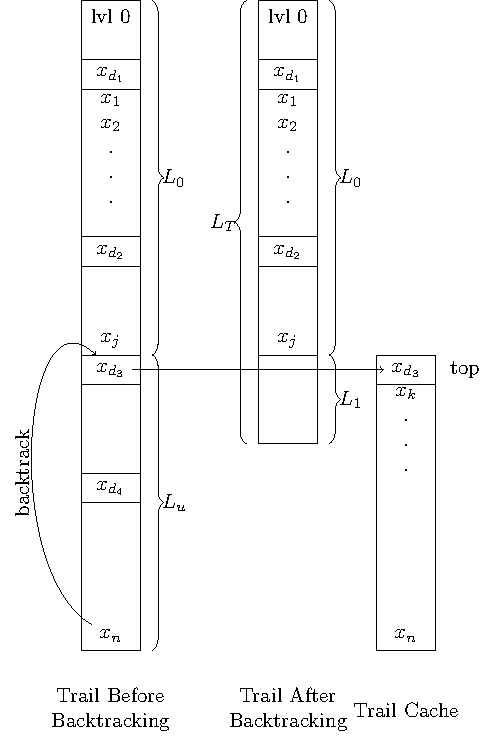
\includegraphics[scale=0.7]{figures/trail_diagram.pdf}\caption{Storing into a trail cache after backtracking.}\end{figure}

\subsection{Restoring the trail cache}
We will base trail saving on the following critical invariant. If the
top of the trail cache becomes true at any point, even after an
arbitrary number of decisions and propagations have been made since
the last backtrack, the set of literals on the trail cache after the
top and up to but excluding the next literal with a null reason is
still implied by the current trail. The top of the trail cache can
become true either by decision or unit propagation, and this invariant
still holds.\newline

\textit{Proof 1} We will refer to the set of literals that become
unassigned during the backtrack after conflict analysis has taken
place as $L_u$, and will refer to the rest of the trail that remains
assigned as $L_0$. We will refer to all of the literals that get
placed on the trail after $L_0$ during subsequent propagations and
decisions as $L_1$. We will refer to the current trail $L_0 \cup L_1$
as $L_T$. The trail cache will contain the literals in $L_u$ ordered
by their appearance on the old trail. Let $L_c[i]$ denote the set of
the first i literals on the trail cache. Let $L_c[top]$ be the top of
the old trail, which gets updated as parts of the trail cache get
restored.

The $i$th literal on the trail cache is implied by
$L_0 \cup L_c[i-1]$, as long as the $i$th literal has a non-null
reason, since $L_0 \cup L_c[i-1]$ had forced $L_c[i]$ on the previous
trail. $L_0 \subseteq L_T$, since $L_T = L_0 \cup L_1$. Therefore, the
$i$th literal on the trail cache is also implied by
$L_T \cup L_c[i-1]$.

Assume $L_c[top]$ is true, which means that
$L_c[0], ..., L_C[top] \subseteq L_1 \subseteq L_T$. Then, from above,
every literal on the trail cache up to but excluding the next literal
with a nun-null reason would be implied. $\blacksquare$\newline

Once the backtrack has been completed and the solver resumes with
decisions and propagations, we will attempt to restore parts of the
trail cache automatically during propagation to make it faster by
using the invariant stated above. Each time the propagation routine is
about to propagate a new literal, we first check the top of the trail
cache to determine its truth value. If that literal's truth value is
already true, we assign all of the literals that come after it on the
trail cache to be true up until (and excluding) the next literal with
a null reason.

A potentially quadratic speedup can be realized during the propagation
of these literals since they are being propagated as a set, rather
than one at a time, as argued in \cite{DBLP:conf/sat/HickeyB19,DBLP:journals/jair/Gent13}. Restoring literals from the trail cache
automatically not only leads to quicker propagation of future
literals, but also means that the propagation routine has less work to
do as it searches for new watchers in clauses on watchlists. All of
the reasons attached to these literals that are automatically restored
will now be satisfied, thus the propagation routine can skip over them
rather than having to access each of them potentially multiple times
to find they are unit.

If at any time the top of the trail cache is a literal $l$ with a
non-null reason whose truth value is already false, we determine a
conflict has occurred with the conflict clause being $l$'s reason from
the trail cache. This is because we know from Proof 1 that $l$ is
implied to be true at this point by the reason on the trail cache
(i.e., the reason on the trail cache is unit), but $\lnot l$ was also
previously assigned to be true, therefore we have a conflict. This
leads to a third potential speed up, since a conflict has been
detected and none of the pending propagations have to be
completed. Since trail saving can sometimes save hundreds or thousands
of literals at a time, the number of propagations required to detect a
conflict could be very costly.

% \begin{algorithm}
%   	\TitleOfAlgo{propagate()}
% 	\begin{algorithmic}[1]
%         \While{queue not empty}
%         \Statex
%         \State restoreTrailCache()
%         \Statex
%         \State $l := $ next literal on queue
%         \For{each clause $c \in $ watchlist($\neg l$)}
% 		\For{each literal $x \in c$}
%         \If{$val($x$) \neq$ false and x is not already a watcher of c}
%         \State let $x$ be a watcher of $c$ and add $c$ to watchlist($\neg x$)
%         \State break
%         \EndIf
% 		\EndFor
% 		\If{no new watcher was found}
%         \If{other watcher $x_2$ of $c = $ false}
%         \State return c as conflict
%         \ElsIf{other watcher $x_2$ of $c$ is unassigned}
%         \State enqueue $x_2$
%         \EndIf
% 		\EndIf
%         \EndFor
%         \EndWhile
% 	\end{algorithmic}
% \end{algorithm}

% \begin{algorithm}
%   	\TitleOfAlgo{restoreTrailCache()}
% 	\begin{algorithmic}[1]
%         \If{trail saving turned on}
% 		\State{let tc $=$ top of trail cache}
% 		\If{val(top of trail cache) $=$ true}
%         \While{trail cache not empty}
%         \State{move top of trail cache (tc) to next literal}
%         \If{reason(tc) is null}
%         \State{break}
%         \ElsIf{val(tc) $=$ false}
%         \State{return conflict with reason(tc)}
%         \ElsIf{val(tc) $=$ unassigned}
%         \State{enqueue tc with reason reason(tc)}
%         \EndIf
%         \EndWhile
% 		\EndIf
%         \EndIf
% 	\end{algorithmic}
% \end{algorithm}

\subsection{Enhancements}

In the standard version of trail saving outlined above, the trail
cache needs to be deleted after each backtrack in order to make room
for the new backtracked literals to be cached. The first enhancement
to trail saving is to keep the trail cache intact instead of clearing
it before each backtrack, and to add the literals that will be
backtracked over to the beginning of the already existing trail
cache. In order to preserve soundness, we must add the literals from
the current backtrack to the beginning of the trail cache, such that
the trail cache has as its prefix the literals which are being
backtracked over, and as its suffix the previous trail cache. \newline

\textit{Proof 2} We will use all of the same set names as Proof 1 and
also refer to the set of literals on our previous trail cache as
$L_{pc}$. We concatenate the literals in $L_{pc}$ to the end of $L_c$
to get $L_{sc}$. We know that $L_{pc}$ is a valid trail cache for
$L_0 \cup L_u$. If we reach the end of $L_c$ without any conflicts, we
know that $L_u \subseteq L_T$. Since $L_0 \subseteq L_T$, then
$L_u \cup L_0 \subseteq L_T$ and therefore $L_{pc}$ is a valid trail
cache for $L_T$. $\blacksquare$\newline

In order for the previous trail cache to be of any use, one must
actually never store the last level of the current trail to the trail
cache at all, since a learnt clause prevents the last level from being
duplicated in the future. If any part of the previous trail cache was
used to construct this last level, it must also be discarded from the
previous trail cache before the previous trail cache is concatenated
to the end.

When concatenating trail caches together as above, it is important to
note that the running trail cache can grow indefinitely. The trail
cache can be trimmed periodically in the following way. Traverse down
the trail cache and whenever a literal appears more than once, delete
its entry in the trail cache. Whenever a literal $x$ appears whose
complement $\lnot x$ has already appeared on the trail cache, $x$
should be deleted and everything remaining until the end of the trail
cache should be deleted (in order to keep the trail cache free of
conflicts).  We decided to trim the trail cache whenever its size
exceeded twice the total number of variables in the SAT instance, as
that is what worked best in preliminary experiments.\newline

The next enhancement to trail saving is to scan the trail cache to
check if there is a literal that is already assigned false within some
limit. The limit we found worked best is to scan the trail until the
third null reason is found (i.e. "looking ahead 2 decisions"). If a
literal that is already assigned false is found, we know that we are
guaranteed to have a conflict in the near future, and we force the SAT
solver's subsequent decisions to come from the trail cache instead of
using the regular variable selection heuristic.

Sometimes using trail saving to automatically restore literals with
their previous reasons will lead to a literal getting a reason that is
"worse" (in terms of number of literals, but one could use a different
metric) than the reason it would have ended up with under normal
propagation (i.e. without trail saving). The last enhancement we made
to trail saving was to stop restoring literals from the old trail as
soon as we hit a reason that we suspected might be "bad". For this, we
kept a running mean and standard deviation of the length of all
reasons used in the solver so far, and decided to stop restoring from
the trail whenever we hit a reason that was greater in length than two
standard deviations above the mean length. This way, when normal
propagation resumes, we give it a chance to find a better reason than
the one that trail saving had stored from the last descent down the
trail.

Another potential enhancement one could use is to use the trail cache
to try to learn a second clause automatically when the solver reaches
a conflict. However, we did not find a way to implement this to make
it beneficial and the number of levels we have to scan for a second
conflict would have to be more than the number of levels we already
look ahead on each decision (when the solver is not under conflict).

\section{Related Work}
\subsection{Trail Saving for Assumption-Based SAT}
Trail saving was briefly introduced in the context of assumption-based
SAT \cite{DBLP:conf/sat/HickeyB19} in order to speed up the
propagation of the assumptions each time the solver backtracked past
the assumption levels. Note that the process is the same, but it only
works to restore the propagants and implicants of the assumptions and
only after a learnt unit clause. Becuase the number of propagants and
implicants of the assumptions tends to become dominated by the number
of assumptions in the applications it was tested on, the technique did
not yield a significant improvement. It would be interesting to
combine the extended version of trail saving outlined in this paper
with trail saving over the assumptions to see if that could produce
better results.

\subsection{Comparison to Chronological Backtracking}
As mentioned earlier, chronological backtracking also achieves some of
the theoretical speedups that trail saving achieves. One advantage of
chronological backtracking is that it does not require any caching of
the trail or accessing such a cache during propagation; it simply
leaves a vast portion of the trail intact rather than backtracking all
the way to the conflict level. Chronological backtracking will also
speed up propagations slightly more than trail saving, because it
leaves more literals assigned at once which leads to clauses being
detected as unit more quickly.

One disadvantage that chronological backtracking has compared to trail
saving is that it doesn't allow the search as much flexibility to jump
out of local neighbourhoods, as the common variable selection
heuristics tend to depend on
\cite{DBLP:conf/dac/MoskewiczMZZM01,DBLP:conf/sat/2015,DBLP:conf/sat/LiangGPC16}. Because
chronological backtracking leaves a large portion of the trail
assigned, it will behave similarly to how the solver would behave if
it was to force the decisions that do occur within this large portion
of literals, whereas trail saving does not force any decisions. As
variable selection heuristics become more refined, it is likely that
adhering to them will become more crucial to performance.

Another disadvantage is that, because propagation is not performed at
every decision level, literals that remain assigned during
chronological backtracking (but otherwise would have been unassigned)
do not have a chance to move their decision levels up. An example of
this is when the solver was supposed to backtrack over a literal that
would end up being unit propagated at level 0, but stays assigned at
its current decision level when chronological backtracking is
used. This could potentially effect the lbd score or length of the
learnt clause that gets generated at the next conflict. Additionally,
chronological backtracking breaks the invarant that all literals
appear on the trail in monotonically increasing order by decision
level, which makes its implementation slightly more complicated.

\section{Experiments and Results}
For the version of cadical published in
\cite{DBLP:conf/sat/MohleB19}chronological backtracking gives solves 6
more problems and has a lower Par-2 score by a decent margin. When
adding trail saving and all enhancements to the default
non-chronological version of cadical, we end up solving 4 more problems
and the Par-2 score goes decreases by a margin not as good as that
produced by the non-chronological backtracking version. The trail saving
versions improve on the standard non-chronological backtracking but do
slightly worse than the chronological backtracking versions.

For the latest version of cadical that we downloaded as of January 1,
2020, chronological backtracking (set to default parameters)
interestingly makes the solver perform worse than standard
non-chronological backtracking does. This shows that not all solvers
will benefit from chronological backtracking; it depends on the solver's
mix of heuristics and may require fine-tuning the parameters associated
with chronological backtracking. However, after implementing trail
saving and enhancements on top of this version of cadical with
non-chronological backtracking, the solver performs roughly the same as
it does with standard non-chronological backtracking, and does not
suffer a slow down as chronological backtracking appears to.

For MapleSat, chronological backtracking makes a significant improvement
on MapleLCMDist both in terms of total number of problems solved and
Par-2 score. Similarly, trail saving implemented on top of MapleLCMDist
with non-chronological backtracking receives a similarly significant
improvement in terms of total instances solved and Par-2 score, and
actually outperforms chronological backtracking on both measures.

\begin{figure}
    \begin{tabular}{|l|l|l|l|l|l|}
      \hline
      & Total Solved & SAT & UNSAT & Par-2 (x 10\textasciicircum{}6 s) \\ \hline
      cadical                  & 532          & 314 &  218  & 3.220                             \\ \hline
      cadical\_chrono          & 525          & 308 &  217  & 3.269                             \\ \hline
      cadical\_trail           & 529          & 310 &  219  & 3.248                             \\ \hline
      cadical\_trail\_enhanced & 531          & 313 &  218  & 3.216                             \\ \hline
    \end{tabular}
    \caption{Table of results for cadical, version pulled from github as of January 1, 2020.}
\end{figure}

\begin{figure}
    \begin{tabular}{|l|l|l|l|l|l|}
      \hline
      & Total Solved & SAT & UNSAT & Par-2 (x 10\textasciicircum{}6 s) \\ \hline
      cadical                  & 492          & 289 &  203  & 3.5020                            \\ \hline
      cadical\_chrono          & 498          & 292 &  206  & 3.4400                            \\ \hline
      cadical\_trail           & 493          & 290 &  203  & 3.5228                            \\ \hline
      cadical\_trail\_enhanced & 496          & 292 &  204  & 3.4847                            \\ \hline
    \end{tabular}
    \caption{Table of results for cadical or "chrono", version published in \cite{DBLP:conf/sat/MohleB19}.}
\end{figure}

\begin{figure}
    \begin{tabular}{|l|l|l|l|l|l|}
      \hline
      & Total Solved & SAT & UNSAT & Par-2 (x 10\textasciicircum{}6 s) \\ \hline
      maple           & 458          & 259 &  199  & 3.797                             \\ \hline
      maple\_chrono   & 470          & 271 &  199  & 3.690                             \\ \hline
      maple\_trail    & 472          & 271 &  201  & 3.694                             \\ \hline
      maple\_enhanced & 473          & 277 &  195  & 3.667                             \\ \hline
    \end{tabular}
    \caption{Table of results for MapleLCMDist.}
\end{figure}
\clearpage

\section{Future Work}

With more clever data structures the efficiency of restoring the trail
could be improved. There are a number of parameters which can be
tuned, including how often to refresh the trail, how large the cutoff
point for rejecting "long" reasons should be, how long to wait to
prune the trail cache if one is appending multiple trail caches
together, how far to look ahead on the trail cache for conflicts (in
terms of number of decisions or total number of literals). We only
experimented with a few different settings of these parameters that
made sense, but more careful fine-tuning of these parameters could
further enhance the effectiveness of the technique. There are
potentially other techniques one could use a trail cache for,
including inprocessing steps that involve probing. A look down the
trail cache is an incomplete but very fast way to do a probing step,
as opposed to propagation. It is also possible that trail saving and
chronological backtracking could be combined in some way to produce
even better results.

\bibliography{sat}{}
\bibliographystyle{splncs04}
\end{document}

\iffalse \textit{Example 1} Suppose the literal $y$ can be restored
from the trail cache, and its reason clause $cr$ contains the literals
${y \lnot x_1, \lnot x_2, ..., \lnot x_n}$. This means that
$x1, ..., x_n$ have become true and are currently on the
trail. Suppose $x_n$ is the most recent literal on the trail and
Without trail saving, the propagation routine will have to access $cr$
from the watchlist of one of the literals $\blacksquare$\newline

\textit{Example 1} Suppose the literals $x_1, ... x_n$ are on the
trail cache, with none of them having a null reason, and $x_1$ becomes
true (e.g., the solver makes a decision for $x_1$ to be true). Then,
$x_2, ... x_n$ are implied by the current trail. Now we will examine
the propagation of a clause c which consists of the literals
$l, \lnot x_1, \lnot x_2, ..., \lnot x_n$ with and without trail
saving. Assume $l$ and $\lnot x_1$ are the current watched literals.

Without trail saving, $\lnot x_1$ becomes false and a new watcher is
searched for and found 1 literal later, $\lnot x_2$, and then
$\lnot x_1$ and $\lnot x_2$ are swapped. Next $\lnot x_2$ becomes
false, a new watcher is searched for and found 2 literals later,
$\lnot x_3$, and then $\lnot x_2$ and $\lnot x_3$ are swapped. This
process will continue until all $x_n$ literals are false, c becomes
unit, and $l$ becomes forced to be true. This propagation took
$1 + 2 + ... + n$ searches through clause c, for a total of $O(n^2)$
searches.

With trail saving, $x2, ... x_n$ are all assigned to be true as soon
as $x_1$ is made true, so immediately the values of literals
$\lnot x_1, ..., \lnot x_n$ in c are false. During propagation, a new
watcher is searched for to replace $\lnot x_2$, n literals are
saerched over without finding any, thus c is detected as unit and $l$
becomes forced to be true. This propagation took $O(n)$ searches
through clause c. $\blacksquare$\newline \fi

\iffalse
\begin{figure}\includegraphics[scale=0.8]{figures/cactus_cadical.pdf}\caption{\small{Comparison
        of run times for versions of cadical. cadical is without
        chronological backtracking, cadical-chrono is with
        chronological backtracking, cadical-trail is with the first
        version of trail saving, cadical-trail-2levels-ahead is the
        trail saving with all enhancements added.}}\end{figure}
\begin{figure}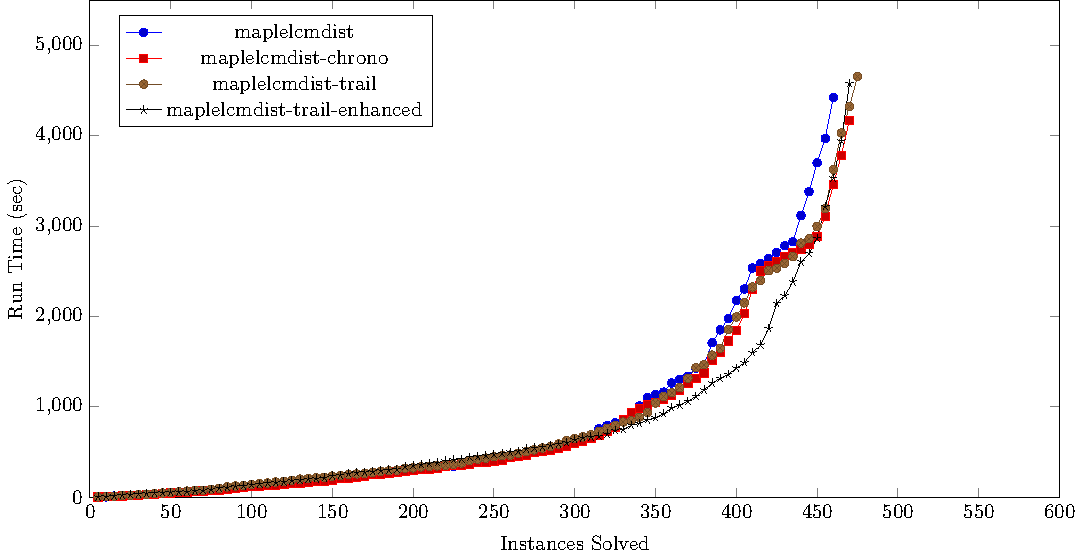
\includegraphics[scale=0.8]{figures/cactus_maple2.pdf}\caption{\small{Comparison
        of run times for versions of MapleSAT. maplelcmdist is from
        the 2017 SAT Competition, maplelecmdist-chrono is with
        chronological backtracking (2018 SAT Competition),
        maplelcmdist-trail is with the first version of trail saving,
        maplelcmdist-trail-enhanced is with trail saving and all
        enhancements added.}}\end{figure}
\begin{figure}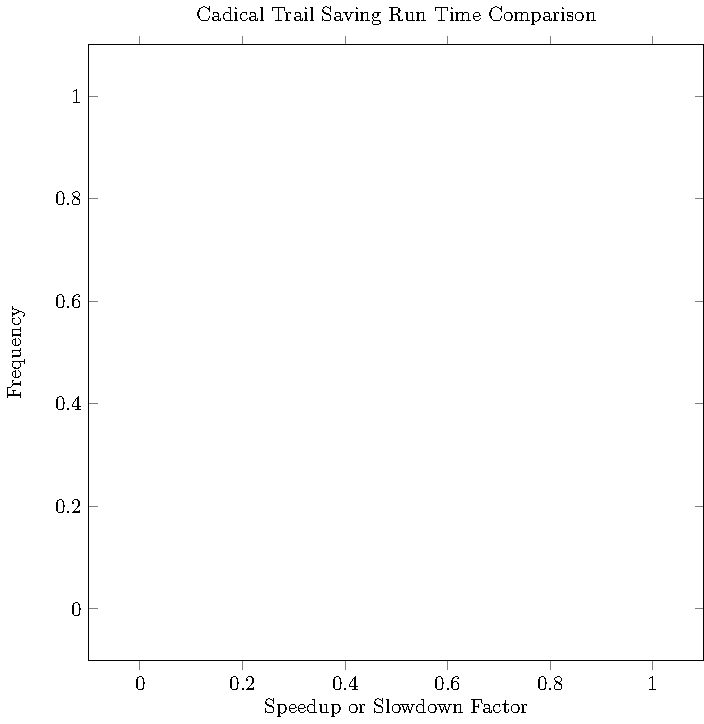
\includegraphics[scale=0.8]{figures/test.pdf}\caption{}\end{figure}
\begin{figure}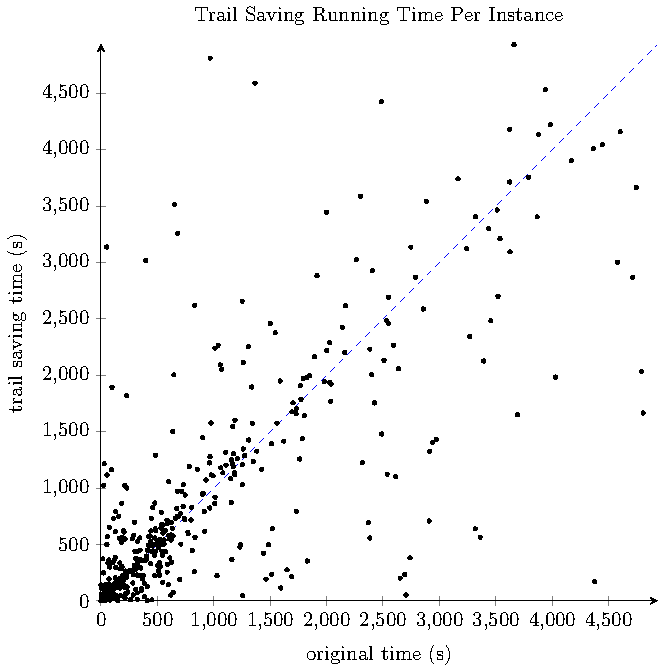
\includegraphics[scale=0.8]{figures/test2.pdf}\caption{}\end{figure}
\fi
\iffalse
\begin{figure}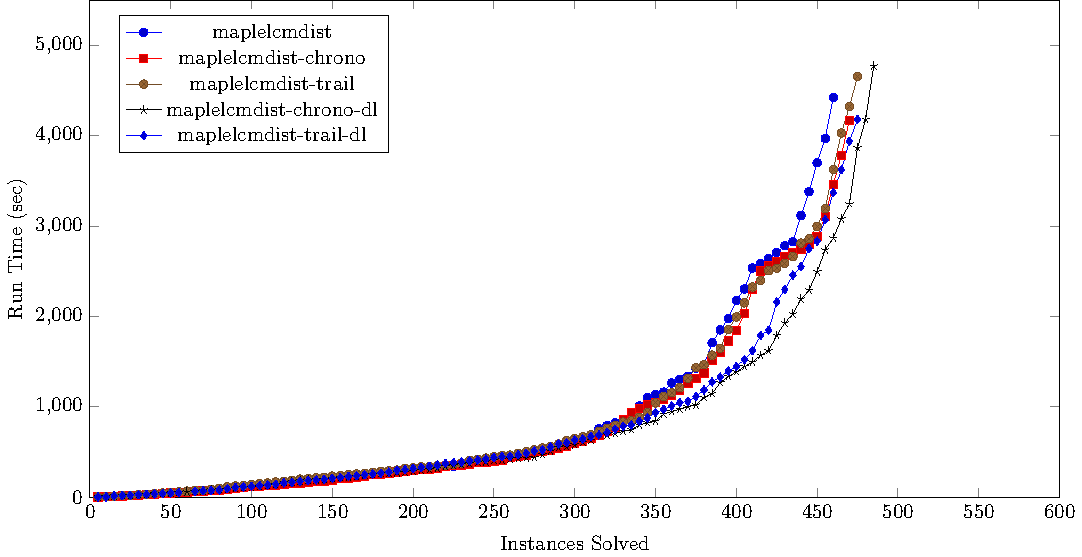
\includegraphics[scale=0.8]{figures/cactus_maple.pdf}\caption{\small{Comparison
        of run times for versions of MapleSAT. maplelcmdist is from
        the 2017 SAT Competition, maplelecmdist-chrono is with
        chronological backtracking (2018 SAT Competition),
        maplelcmdist-trail is with the first version of trail saving,
        maplelcmdist-chrono-dl is with chronological backtracking and
        duplicate learnts (2019 SAT Competition),
        maplelcmdist-trail-dl is with trail saving and duplicate
        learnts}}\end{figure}
\fi

\iffalse
\begin{figure}[t]
    \begin{center}
        \fss{9pt}{10pt}
        \setlength\tabcolsep{1pt}
        \begin{tabular}{| p{4.2cm} | c | c | c | c | c | c | c | c |}
          \hline
          & \multicolumn{4}{|c|}{Total} & \multicolumn{2}{|c|}{Unweighted} & \multicolumn{2}{|c|}{Weighted} \\ \hline
          & MaxHS & +/- & \hspace{1pt} RC2 \hspace{1pt} & +/- & MaxHS & \hspace{1pt} RC2 \hspace{1pt} & MaxHS & \hspace{1pt} RC2 \hspace{1pt} \\ \hline
          original & 6052 & 0/0 & 6030 & 0/0 & 3940 & 3993 & 2112 & 2037 \\ \hline
          enqueue assumptions as set & 6131 & 114/35 & 6081 & \hspace{0.5pt} 99/48 \hspace{0.5pt} & 3995 & 4032 & 2136 & 2049 \\ \hline
          enqueue assumptions as set + \newline save literals after learnt units & 6136 & 120/36 & 6079 & \hspace{0.5pt} 95/46 \hspace{0.5pt} & 3991 & 4030 & 2145 & 2049 \\ \hline
          enqueue assumptions as set + \newline save literals after learnt units + \newline save literals from last invocation & 6138 & 115/29 & 6080 & \hspace{0.5pt} 92/42 \hspace{0.5pt} & 3989 & 4030 & 2149 & 2050 \\ \hline
        \end{tabular}
    \end{center}
    \caption{Number of \maxsat instances solved by MaxHS and RC2 using
      different extensions of the underlying \sat solver. The +/- column shows
      the number of instances gained/lost vs the original.}
    \label{fig:nsolved}
\end{figure}
\fi
